\section{Werner State and Conditional Entropies}
Let's now take one of the most well-known and widely used states when studying conditional entropies, called Werner states. Werner, wrote down this class of states at \cite{werner1989quantum} in order to create entangled states that don't violate Bell's inequalities. Experimental demonstrations of Werner states is an active reasearch area for the last twenty years(\cite{zhang2002experimental}\cite{cinelli2004parametric}).
In our calculation we will use the theoretical form of \cite{pittenger2000note} and all the information related to its separability criteria. Specifically is noted that:
\begin{equation}
W^{\left[d^{n}\right]}(s)=(1-s) \frac{1}{d^{n}} I+s|\Psi\rangle\langle\Psi|
\label{wernerstate}
\end{equation}
where $s$ is a free parameter, $d$ is the dimension of the qudits, $n$ is the number of qudits, $\ket{\Psi}$ is an  entangled state and $I$ is the identity matrix for the composed Hilbert space. It is proven in \cite{pittenger2000note} that the state   $W^{\left[d^{n}\right]}(s)$ is fully separable if and only if $s \leq\left(1+d^{n-1}\right)^{-1}$.
We take the simplest case of $d=2$, $n=2$ and $\ket{\Psi}=(\ket{00}+\ket{11})/\sqrt{2}$ as prescribed. Thus, according to \cite{pittenger2000note} this state is separable iff $s \leq 1/3$:
\begin{align}
W &=\frac{1-s}{4}I_{4}+\frac{s}{2}(\ket{00}\bra{00}+\ket{11}\bra{11}+\ket{11}\bra{00}+\ket{00}\bra{11})\\[0.5em]&=
\left(
\begin{array}{cccc}
 (1+s)/4 & 0 & 0 & s/2 \\
 0 & (1-s)/4 & 0 & 0 \\
 0 & 0 & (1-s)/4 & 0 \\
 s/2 & 0 & 0 & (1+s)/4 \\
\end{array}
\right)
\label{wernerstate}
\end{align}
Let's calculate. Firstly, we trace out the subsystem B. It is easily done if we expand $I$ using the properties of the complete orthonormal set in standard tensor product basis(\cite{ballentine2014quantum}):
\begin{equation*}
\sum_{i}\left|\phi_{i}\right\rangle\left\langle\phi_{i}\right|=I
\end{equation*}
thus in our case:
\begin{equation*}
I_{4}=|11\rangle \langle11|+|00\rangle \langle00|+|10\rangle \langle10|+|01\rangle \langle01|
\end{equation*}
Hence:
\begin{align}
W^A &= \Tr_B (W) \nonumber \\[0.5em]
&= \Tr_B \big(\frac{1+s}{4}\ket{00}\bra{00}+\frac{1+s}{4}\ket{11}\bra{11} +\frac{1-s}{4}\ket{01}\bra{01}+\frac{1-s}{4}\ket{10}\bra{10} \nonumber \\[0.5em]&+\frac{s}{2}\ket{00}\bra{11}+\frac{s}{2}\ket{11}\bra{00} \big) \nonumber \\[0.5em]
&= \Tr_B \big(\frac{1+s}{4}|0\rangle \langle0|\otimes|0\rangle \langle0|+\frac{1+s}{4}|1\rangle \langle1|\otimes|1\rangle \langle1|  +\frac{1-s}{4}|0\rangle \langle0|\otimes|1\rangle \langle1| \nonumber \\[0.5em] &+\frac{1-s}{4}|1\rangle \langle 1|\otimes|0\rangle \langle0|+\frac{s}{2}|0\rangle \langle1|\otimes|0\rangle \langle1|+\frac{s}{2}|1\rangle \langle0|\otimes|1\rangle \langle0|
\big) \nonumber \\[0.5em]
&=\frac{1+s}{4}|0\rangle \langle0|\otimes \Tr \big( |0\rangle \langle0| \big)+\frac{1+s}{4}|1\rangle \langle1|\otimes \Tr \big( |1\rangle \langle1| \big)+\frac{1-s}{4}|0\rangle \langle0|\otimes \Tr \big(|1\rangle \langle1|\big) \nonumber \\[0.5em] &+\frac{1-s}{4}|1\rangle \langle 1|\otimes \Tr \big(|0\rangle \langle0| \big)+\frac{s}{2}|0\rangle \langle1|\otimes \Tr \big( |0\rangle \langle1| \big)+\frac{s}{2}|1\rangle \langle0|\otimes \Tr \big( |1\rangle \langle0|
\big) \nonumber \\[0.5em]
&= \frac{1+s}{4}\ket{0}\bra{0}+\frac{1+s}{4}\ket{1}\bra{1}+\frac{1-s}{4}\ket{0}\bra{0}+\frac{1-s}{4}\ket{1}\bra{1}
\nonumber \\[0.5em] &=
\frac{1}{2}\ket{0}\bra{0}+\frac{1}{2}\ket{1}\bra{1}
\nonumber \\[0.5em] &= I_{2}/2=
\left( \begin{array}{cccc}
 1/2 & 0  \\
 0 & 1/2 \\
\end{array}
\right)
\end{align}
Now let us eigen-decompose the state \eqref{wernerstate} in order to apply \propref{spectraltheorem}. We find the eigenvalues and eigenvectors of $W$:
\begin{equation}
\lambda_1=\frac{1-s}{4},\:  \lambda_2=\frac{1-s}{4},\:  \lambda_3=\frac{1-s}{4},\:  \lambda_4=\frac{1+3s}{4}, 
\end{equation}
\begin{equation}
v_1=\left(
\begin{array}{c}
 -1 \\
 0\\
 0\\
 1 \\
\end{array}
\right),
\:  v_2=\left(
\begin{array}{c}
 0 \\
 0\\
 1\\
 0 \\
\end{array}
\right),
\:  v_3= \left(
\begin{array}{c}
 0 \\
 1\\
 0\\
 0 \\
\end{array}
\right),\:  v_4= 
\left(
\begin{array}{c}
 1 \\
 0\\
 0\\
 1 \\
\end{array}
\right)
\end{equation}
Hence the modal matrix is:
\begin{equation}
M=\left(
\begin{array}{cccc}
 -1 & 0 & 0 & 1 \\
 0 & 0 & 1 & 0 \\
 0 & 1 & 0 & 0 \\
 1 & 0 & 0 & 1 \\
\end{array}
\right)
\end{equation}
which gives:
\begin{equation}
det(M)=2.
\end{equation}
As a result:
\begin{equation}
M^{-1}=
\left(
\begin{array}{cccc}
 -1/2 & 0 & 0 & 1/2 \\
 0 & 0 & 1 & 0 \\
 0 & 1 & 0 & 0 \\
 1/2 & 0 & 0 & 1/2 \\
\end{array}
\right)
\end{equation}
While the diagonal matrix:
\begin{equation}
D=\left(
\begin{array}{cccc}
(1-s)/4 & 0 & 0 & 0 \\
 0 & (1-s)/4 & 0 & 0 \\
 0 & 0 & (1-s)/4 & 0 \\
 0 & 0 & 0 & (3s+1)/4 \\
\end{array}
\right)
\end{equation}
So we have decomposed $W$ as:
\begin{equation}
W=MDM^{-1}.
\end{equation}

\subsection{von Neumann case}
\noindent
According to \eqref{condent} and \propref{spectraltheorem} we find the vonNeumann entropy for $W$ and $W^A$:
\begin{align}
S(W)&=-\Tr \big[ F(W) \big]
\nonumber \\[0.5em] &= -\Tr \big[F(MDM^{-1})\big] \nonumber \\[0.5em] &= -\Tr \left[ M
\left(
\begin{array}{cccc}
F\big((1-s)/4\big) & 0 & 0 & 0 \\
 0 & F\big((1-s)/4\big) & 0 & 0 \\
 0 & 0 & F\big((1-s)/4\big) & 0 \\
 0 & 0 & 0 & F\big((3s+1)/4\big) \\
\end{array}
\right)
M^{-1} \right]
\nonumber \\[0.5em] &=
\frac{3}{4} (s-1) \log \left(\frac{1-s}{4}\right)-\frac{1}{4} (3 s+1) \log \left(\frac{1}{4} (3 s+1)\right)
\end{align}
while:
\begin{align}
S(A)=S(W^A)&=-\Tr \big(W^A \log W^A \big) \nonumber \\[0.5em] 
&=-\Tr\left[\left( \begin{array}{cccc}
 F(1/2) & 0  \\
 0 & F(1/2) \\
\end{array}
\right) \right]
\nonumber \\[0.5em] &=-\Tr\left[\left( \begin{array}{cccc}
 -(\log 2)/2 & 0  \\
 0 & -(\log 2)/2 \\
\end{array}
\right) \right]
\nonumber \\[0.5em] &= \log2
\end{align}
Hence the conditional entropy is:
\begin{align}
S(B|A)_{W}&=S(AB)-S(A)
\nonumber \\[0.5em] &= S(W)-S(W^A)
\nonumber \\[0.5em] &= 
\frac{3}{4} (s-1) \log \left(\frac{1-s}{4}\right)-\frac{1}{4} (3 s+1) \log \left(\frac{1}{4} (3 s+1)\right)-\log (2)
\end{align}
Let's plot:
\begin{figure}[H]
\label{figure2}
\begin{center}
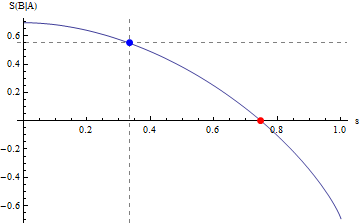
\includegraphics[scale=0.8]{figures/conditional_vonNeumann_Werner.png}
\caption{The blue point $B$ has the coordinates $(1/3,0.549306)$ and the red point $R(0.747614,0)$ which was found via numerical methods. The diagram clearly illustrates that the state $W$ while entangled($s\geq 1/3 $) has positive quantum conditional entropy, a fact emphasized by many sources(for example at \cite{nielsen2001separable}). This particular example becomes negative for $s  \gtrsim 0.747614$. A similar diagram can be found in \cite{patro2017non}.}
\end{center}
\end{figure}
\subsection{Tsallis case}
\noindent
The Tsallis entropy for the whole state as defined:
\begin{align}
T(q;W) &= \frac{1}{1-q} \left\{ \Tr \left[ t(q;W) \right] -1   \right\} \nonumber \\[0.5em]
&= \frac{1}{1-q} \left\{ \Tr \left[ t(q;MDM^{-1}) \right] -1   \right\} \nonumber \\[0.5em]
&=\frac{1}{1-q} \left\{ \Tr \left[
M
\left( \begin{array}{cccc}
 t(q;\frac{1-s}{4}) & 0 & 0 & 0 \\
 0 & t(q;\frac{1-s}{4}) & 0 & 0 \\
 0 & 0 & t(q;\frac{1-s}{4}) & 0 \\
 0 & 0 & 0 & t(q;\frac{3s+1}{4}) \\
\end{array}
\right)
M^{-1}
\right]-1
\right\}
\nonumber\\[0.5em]
&=\frac{2^{-2 q} (1-s)^q+2^{1-2 q} (1-s)^q+2^{-2 q} (3 s+1)^q-1}{1-q}.
\end{align}
For the subsystem A we readily see that:
\begin{align}
T(q;W^A)&= \frac{1}{1-q} \left\{ \Tr \left[ t(q;W^A) \right] -1   \right\} \nonumber \\[0.5em] &= \frac{2^{1-q}-1}{1-q}
\end{align}
From  the quantum conditional Tsallis entropy gives:
\begin{align}
T(B|A)_{W}&=\frac{T(q;W)-T(q;W^A)}{1+(1-q) T(q;W^A)}
\nonumber \\[0.5em] &= \frac{2^{-q-1} \left(-3 (1-s)^q-(3 s+1)^q+2^{q+1}\right)}{q-1}
\label{calccondtsa}
\end{align}
Let's plot for some values of $q$:
\begin{figure}[H]
\label{figure2}
\begin{center}
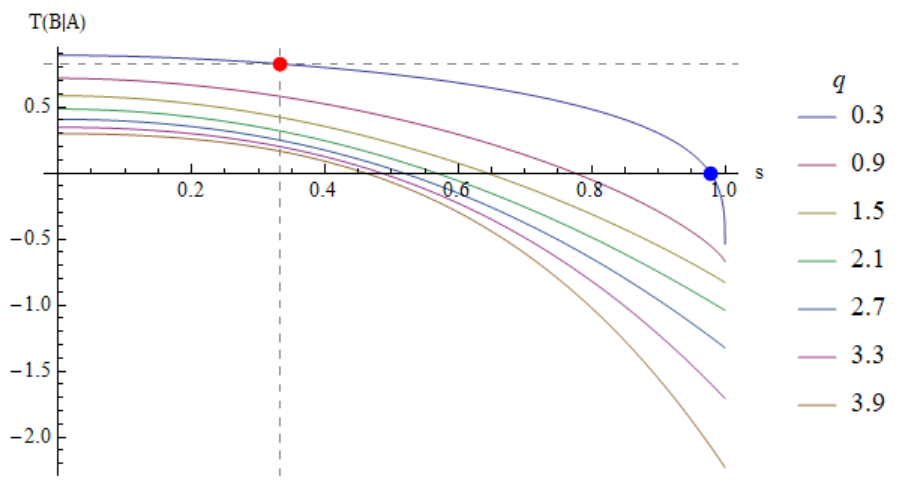
\includegraphics[scale=0.8]{figures/conditional_tsallis_werner.png}
\caption{As an example, blue point $B$ has the coordinates $(0,0.978043)$ and the red point $R(1/3,0.826907)$ which was found via numerical methods. This diagramm again illustrates that the state $W$ while entangled($s\geq 1/3 $) has positive quantum Tsallis conditional entropy for most $q$'s.}
\end{center}
\end{figure}
Let's see how the entanglement limit value of the quantum conditional Tsallis entropy changes with $q$, i.e. the value of $T(B|A)_{W}$ for $s=1/3$. From \eqref{calccondtsa} we get:
\begin{equation}
T(\tfrac{1}{3};B|A)_W= \frac{2^{-q-1} \left(-2^q+2^{q+1}-2^q 3^{1-q}\right)}{q-1}
\end{equation}
and the plot:
\begin{figure}[H]
\label{figure2}
\begin{center}
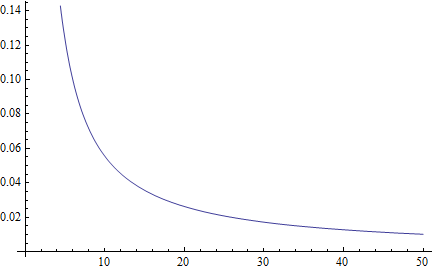
\includegraphics[scale=0.7]{figures/diag1.png}
\caption{We can numerically see in this example that for larger $q$ the entanglement limit value is getting smaller.}\label{figr1}
\end{center}
\end{figure}
\noindent
As always we present the 3Dplot for intuition:
\begin{figure}[H]
\label{figure2}
\begin{center}
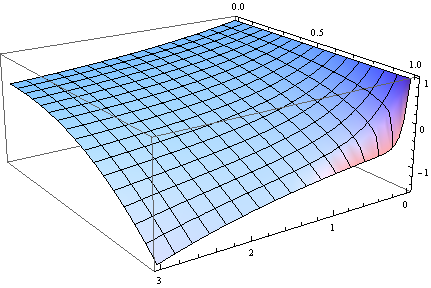
\includegraphics[scale=0.8]{figures/3DplotTsallis.png}\caption{The 3D plot of \eqref{calccondtsa}}
\label{figr2}
\end{center}
\end{figure}
\subsection{Renyi Case}
\noindent
For the total W state we find:
\begin{align}
R(\alpha;W) &= \frac{1}{1-\alpha}\log \left\{ \Tr \left[ r(\alpha;MDM^{-1}) \right] \right\} \nonumber \\[0.5em]
&=\frac{1}{1-\alpha} \log \left\{ \Tr \left[
M
\left(
\begin{array}{cccc}
 4^{-\alpha } (1-s)^{\alpha } & 0 & 0 & 0 \\
 0 & 4^{-\alpha } (1-s)^{\alpha } & 0 & 0 \\
 0 & 0 & 4^{-\alpha } (1-s)^{\alpha } & 0 \\
 0 & 0 & 0 & 4^{-\alpha } (3 s+1)^{\alpha } \\
\end{array}
\right)
M^{-1}
\right] \right\}
\nonumber\\[0.5em]
&=-\frac{\log \left(4^{-\alpha } \left(3 (1-s)^{\alpha }+(3 s+1)^{\alpha }\right)\right)}{a-1}
\end{align}
while for the subsystem:
\begin{align}
R(\alpha;W^A)&= \frac{1}{1-\alpha} \left\{\log \Tr \left[ \left(
\begin{array}{cc}
 2^{-\alpha } & 0 \\
 0 & 2^{-\alpha } \\
\end{array}
\right) \right] \right\} \nonumber \\[0.5em] &= \frac{2^{1-q}-1}{1-q}  \\[0.5em] &=
\frac{\log \left(2^{1-\alpha }\right)}{1-a}
\end{align}
Hence:
\begin{align}
R(B|A)_{W}&=R(\alpha;W)-R(\alpha;W^{A})
\nonumber \\[0.5em] &=
\frac{\log \left(2^{1-\alpha }\right)-\log \left(4^{-\alpha } \left(3 (1-s)^{\alpha }+(3 s+1)^{\alpha }\right)\right)}{\alpha -1}
\label{renyicasecalc}
\end{align}
Let's plot:
\begin{figure}[H]
\label{figure2}
\begin{center}
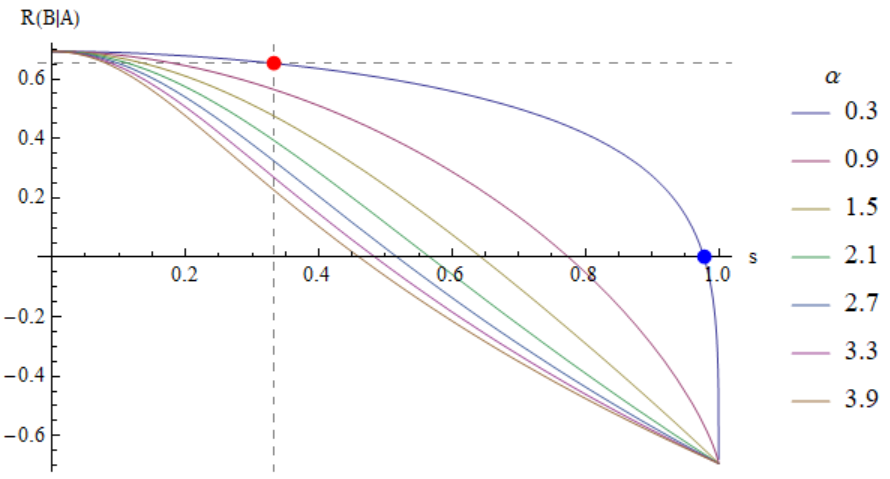
\includegraphics[scale=0.8]{figures/conditional_renyi_werner.png}
\caption{As an example, blue point $B$ has the coordinates $(0,0.978043)$ and the red point $R(1/3,0.65241)$ which was found via numerical methods. This plot again illustrates that the state $W$ while entangled($s\geq 1/3 $) has positive quantum Renyi conditional entropy for most $\alpha$'s.}
\end{center}
\end{figure}
We emphasize, that the identical value of $s$ when Tsallis and Renyi entropies are taken to zero for $\alpha=q=0.3$, is not an accident nor a mistake. It is an example of a general result $T(x ; B \mid A)_{\rho} \geq 0 \quad \Leftrightarrow \quad S(x; B \mid A)_{\rho} \geq 0$ as discussed in \cite{vollbrecht2002conditional}. As with the Tsallis entropy we the entanglement limit value for the quantum conditional Renyi entropy:
\begin{equation}
R(\tfrac{1}{3};B|A)_W=
\frac{\log \left(2^{1-\alpha }\right)-\log \left(4^{-\alpha } \left(2^{\alpha }+2^{\alpha } 3^{1-\alpha }\right)\right)}{\alpha -1}
\end{equation}
and the plot:
\begin{figure}[H]
\begin{center}
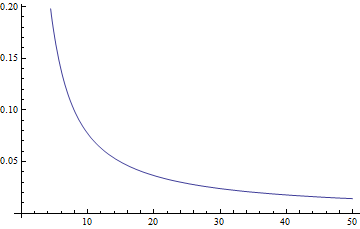
\includegraphics[scale=0.8]{figures/diag2.png}
\caption{We can numerically see in this example that for larger $\alpha$ the entanglement limit value is getting smaller.}
\label{figr3}
\end{center}
\end{figure}
\noindent
The 3-D plot will give:
\begin{figure}[H]
\begin{center}
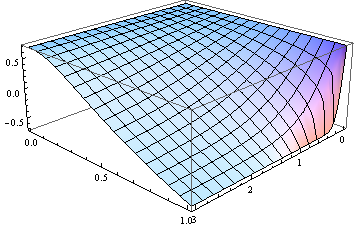
\includegraphics[scale=0.9]{figures/3DplotRenyi.png}
\caption{The 3-D plot of \eqref{renyicasecalc}}
\label{figr4}
\end{center}
\end{figure}